\section{设计概览}

\subsection{设计假设}
在为满足自身需求而设计文件系统时，我们遵循了一些既带来挑战、
也带来机遇的假设。前文已提及一些关键观察；现在将更详细地说明
这些假设。

\begin{itemize}
  \item 系统由许多廉价且经常发生故障的通用组件构建而成。它必须持续
  监控自身，并能在日常运行中检测、容忍组件故障，并从中迅速恢复。
  \item 系统存储数量适中的大文件。我们预计会有数百万个文件，每个文件
  通常为100MB或更大。数GB大小的文件是常见情况，应被高效管理。
  系统必须支持小文件，但无需针对小文件进行优化。\emph{(译者注：因为
  这类存储往往是用来读取或写入大文件的，经典场景是大数据处理)}
  \item 这些文件访问负载主要包括两类读操作：大型流式读取和小型随机读取。
  在大型流式读取中，单次操作通常会读取数百KB，更常见的是读取1MB或更多。
  同一个客户端连续发起的操作，往往会沿着文件中的一段连续区域向前读取。
  小型随机读取通常会在任意offset处读取几KB。注重性能的应用通常会把这些小读
  请求批量处理并排序，使读取位置在文件中稳定向前推进，而不是来回跳转。
  \item 这些文件访问负载还包含许多向文件追加数据的大型顺序写入。典型操作
  大小与读取操作相近。文件写入后很少再次被修改。系统支持在文件任意位置
  进行小写入，但不要求这种操作具有高性能。\emph{(译者认为，因为这类操作本身
  就不是GFS主打，GFS主打大block顺序读写，而不是海量小文件读取，或者随机写，因此不必要被
  优化得很高效)}
  \item 系统必须高效实现明确的语义，以支持多个客户端并发向同一文件追加
  数据。我们的文件常被用作生产者—消费者队列，或用于多路合并。
  数百个生产者每台机器运行一个，会并发向同一文件追加数据\emph{(译者注：经典
  的Fan-In模式，多个客户端向一个文件扇入数据)}。以最小
  同步开销保证原子性至关重要。文件可能稍后才被读取，也可能正被某个
  消费者同时顺序读取。
  \item 高且持续的带宽比低延迟更重要。我们的大多数目标应用都重视以高
  速率批量处理数据；只有少数应用对单次读取或写入的响应时间有严格
  要求。
\end{itemize}

\subsection{接口}
GFS提供了熟悉的文件系统接口，但并未实现POSIX这类标准API。文件按
目录进行层次化组织，并由路径名标识。系统支持常见的创建、删除、打开、
关闭、读取和写入文件操作。

此外，GFS还提供\textbf{snapshot}和\textbf{record append}操作。
\textbf{snapshot}能够以较低成本创建文件或目录树的replica。\textbf{record append}
允许多个客户端并发向同一文件追加数据，同时保证每个客户端单次追加操作的原子性。
\textbf{record append}可以实现多路合并结果，以及允许许多客户端无
需额外加锁便能同时追加数据的生产者—消费者队列。我们发现，这
类文件对于构建大型分布式应用非常有价值。section3.4和section3.3
将分别进一步讨论\textbf{snapshot}和\textbf{record append}。

\begin{figure*}[t]
  \centering
  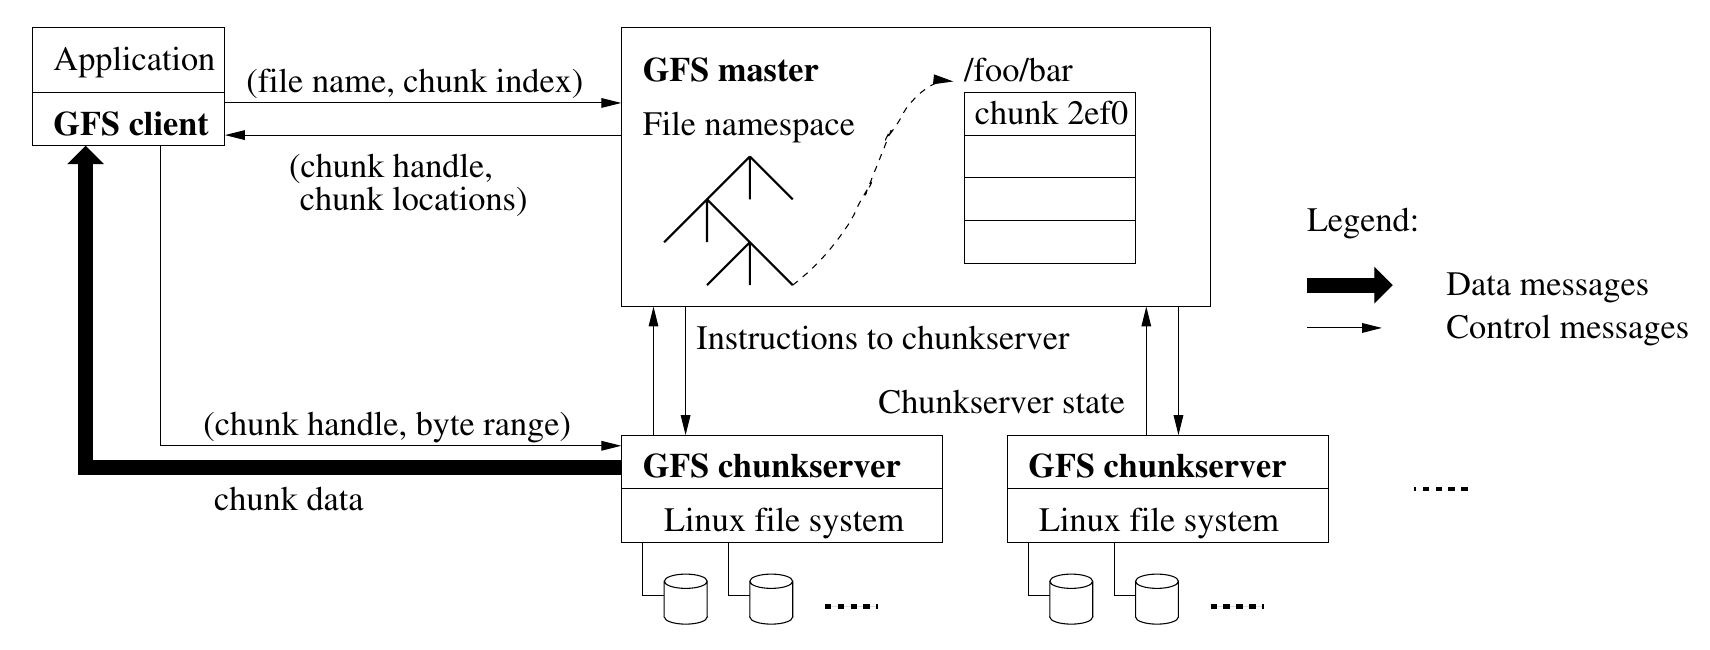
\includegraphics[width=0.96\textwidth]{figures/original/gfs-figure-1-architecture.png}
  \captionsetup{justification=centering}
  \renewcommand{\figurename}{Figure}
  \caption{GFS架构}
  \label{fig:gfs-architecture}
\end{figure*}

\subsection{架构}
如Figure 1所示，一个GFS集群由单个master和多个chunkserver组成，并由
多个客户端访问。它们通常都作为用户态进程的运行在普通的Linux服务器上。
只要机器资源允许，并且能够接受由于运行可能不太稳定的应用程序代码而带
来的可靠性下降，那么在同一台机器上同时运行chunkserver和client是很容易的。
\emph{(译者注：事实上Google的MapReduce机器会和chunkserver混合部署，
目的是尽量减少Map阶段的带宽消耗)}

文件被划分为固定大小的chunk。每个chunk都由master在创建时分配的、
不可变且全局唯一的64位chunk handle标识\emph{(译者注：它不是文件offset，
也不是文件名，也不是磁盘地址，而是master给某个chunk分配的一个64位标识符)}。chunkserver将chunk作为
Linux文件存储在本地磁盘上，并根据chunk handle和字节范围读取或写入
chunk数据。为保证可靠性，每个chunk都会复制到多个chunkserver上。
默认情况下，我们保存3个replica；不过用户可以为文件命名空间的不
同区域指定不同的复制级别。\emph{(译者认为此处指可以给不同的路径树前缀，
设置单独的replica数，比如告诉/critical/这个路径下面的所有子文件都要5 replica)}

master维护所有文件系统元数据，包括命名空间\emph{(译者认为namespace
可以理解成目录树信息)}、访问控制信息、从文件到
chunk的映射，以及chunk的当前位置。它还控制全系统范围的活动，例如
chunk lease管理、孤立chunk的垃圾回收，以及chunk在不同chunkserver之间
的迁移。master会定期通过HeartBeat消息与每个chunkserver通信，向其
发送指令并收集其状态。

每个应用程序中的GFS客户端代码实现了文件系统API，并代表应用程序
与master和chunkserver通信以读写数据。客户端在执行元数据操作时与master
交互，但所有承载数据的通信都会直接发送到chunkserver。我们不提供POSIX
API，因此无需hook到Linux vnode层。

客户端和chunkserver都不缓存文件数据。客户端缓存带来的收益很小，因为
大多数应用会流式遍历超大文件，或其工作集大到无法被缓存。不缓存文件数据
能够消除缓存一致性问题，从而简化客户端和整个系统(不过，客户端会缓存
元数据)。chunkserver也无需缓存文件数据，因为chunk以本地文件形式存储，
Linux的缓冲区缓存已经会将频繁访问的数据保留在内存中。

\subsection{单个主控(master)服务器}
单个master极大简化了我们的设计，并使master能够利用全局信息做出
复杂的chunk放置和复制决策。然而，我们必须尽量减少它参与读取和写入
的程度，以免它成为瓶颈。客户端绝不会经由master读取或写入文件数据。
相反，客户端会询问master应联系哪些chunkserver，并在有限时间内缓存
这些信息，随后直接与chunkserver交互来完成许多操作。

下面结合Figure 1说明一次简单读取的交互过程。首先，客户端根据固定的chunk
大小，将应用程序指定的文件名和字节offset转换为该文件中的chunk索引，
\\\emph{
译者注：chunk索引计算公式：
\[
\left\lfloor \frac{\text{offset}}{64 \times 1024 \times 1024} \right\rfloor
\]}
然后，它向master发送一个包含文件名和chunk索引的请求。master返回相应
的chunk handle及replica位置。客户端使用文件名和chunk索引作为键，缓存
这些信息。

接着，客户端向其中一个replica发送请求，通常会选择距离最近的replica。请求
中包含chunk handle和该chunk内的字节范围。在缓存信息过期或文件被重新
打开之前，对同一个chunk的后续读取不再需要客户端与master交互。

实际上，客户端通常会在同一个请求中查询多个chunk，而master也可以返回
紧随这些chunk之后的chunk信息。这些额外信息几乎不增加成本，却能避免
之后多次客户端与master之间的交互。

\subsection{Chunk大小}
Chunk大小是关键设计参数之一。我们选择了64MB，这远大于典型的
文件系统块大小。每个chunk replica都作为普通Linux文件存储在
chunkserver上，并且只在需要时扩展。延迟(lazy)空间分配避免了内部碎片造成的空间浪费；
而内部碎片可能正是人们反对采用如此大chunk大小的最大理由。\emph{（译者注：
这里作者是在回应大chunk可能带来的空间浪费问题。64MB是chunk的逻
辑上限和管理粒度，并不意味着每创建一个chunk replica就会立刻占用64MB磁盘
空间。由于chunk replica只是普通Linux文件，并且只会随着实际写入而扩展
，因此即使最后一个chunk没有写满，也不会必然浪费完整的64MB空间。
这里的内部碎片指的是固定大chunk可能导致的未使用空间浪费，而不是内存碎片）}

较大的chunk大小具有几个重要优点。第一，同一chunk上的读写只需
在开始时向master请求一次chunk位置信息，因此它减少了客户端与
master交互的需求。对于我们的访问负载，这种减少尤其显著，因为
应用大多顺序读写大文件。即使进行小型随机读取，客户端也能轻松
缓存一个多TB工作集中全部chunk的位置信息。第二，由于客户端更可
能在一个大chunk上执行多次操作，它可以在较
长时间内保持与chunkserver之间的持久TCP连接，从而降低网络开销
\emph{(译者注：这里的意思是，应用通常会顺序访问大文件或其中一段连续区
域。chunk越大，客户端在同一个chunk内连续读写的机会越多，因此更可能复
用同一个chunkserver连接，而不是频繁查询master、切换chunk或重新
建立TCP连接)}
。第三，它减少了存储在master上的元数据规模。这使我们能够将元数据
保存在内存中，进而带来将在section2.6.1讨论的其他优点。

另一方面，即使采用延迟空间分配，大chunk大小也有缺点。一个小文件
只包含少量chunk，可能只有一个。如果许多客户端访问同一文件，存储
这些chunk的chunkserver可能成为热点。实践中，热点并不是主要问题，
因为我们的应用大多顺序读取包含多个chunk的大文件。

然而，在GFS最初被一个批处理队列系统使用时，确实出现了热点：一个
可执行文件被作为单chunk文件写入GFS，随后在数百台机器上同时启动。
存储该可执行文件的少数chunkserver被数百个并发请求压垮。我们通过提高这
类可执行文件的复制因子\emph{(译者注：简单理解为replica数量即可)}，
并让批处理队列系统错开应用
启动时间，解决了这个问题。一种潜在的长期方案是：在这类情况下允许
客户端从其他客户端读取数据。

\subsection{元数据}
master存储三类主要元数据：文件和chunk命名空间、从文件到chunk的
映射，以及每个chunk replica的位置。所有元数据都保存在master的内存中。
前两类元数据(命名空间和文件到chunk的映射)还会通过操作日志持久化。
每次变更都会记录到存放在master本地磁盘、并复制到远程机器上的操作
日志中。使用日志使我们能够简单、可靠地更新master状态，并避免在
master崩溃时出现不一致的风险。
master不会持久化存储chunk位置信息。相反，master会在启动时，以及
每当某个chunkserver加入集群时，向各个chunkserver询问其持有的
chunk。
\\\emph{译者注：master内存结构接近这样}\\
\begin{minipage}{\columnwidth}
{\scriptsize
\begin{verbatim}
Master Memory
│
├── Namespace table
│   ├── "/"             -> 目录metadata
│   ├── "/foo"
│   ├── "/foo/bar"
│   └── "/foo/bar/a.txt"-> 文件metadata
│
├── File-to-chunk table
│   └── "/foo/bar/a.txt"
│       ├── chunk index 0 -> chunk_11
│       ├── chunk index 1 -> chunk_12
│       └── chunk index 2 -> chunk_13
│
├── Chunk metadata table
│   ├── chunk_11
│   │   ├── version number
│   │   ├── lease holder, if any
│   │   └── replica位置 -> [CS1, CS4, CS8]
│   │
│   └── chunk_12
│       ├── version number
│       ├── lease holder, if any
│       └── replica位置 -> [CS2, CS5, CS9]
│
└── Chunkserver state table
    ├── CS1 -> alive, disk usage, chunks it own
    ├── CS2 -> alive, disk usage, chunks it own
    └── CS3 -> alive, disk usage, chunks it own
\end{verbatim}
}
\end{minipage}

\subsubsection{内存数据结构}
由于元数据存储在内存中，master操作速度很快。此外，master能够
方便且高效地在后台定期扫描其全部状态。这种周期性扫描用于实现
chunk垃圾回收、在chunkserver发生故障时重新复制chunk，以及为平衡
各chunkserver之间的负载和磁盘空间使用而迁移chunk。section4.3和
section4.4会进一步讨论这些活动。

这种仅将元数据存储在内存中的方案有一个潜在顾虑：chunk数量以及
整个系统的容量，会受到master可用内存大小的限制。然而在实践中，
这并不是严重限制。对于每个64MB的chunk，master维护的元数据不足
64字节。大多数chunk都是满的，因为大多数文件包含许多chunk，只有最后一个
chunk可能未被完全填满。同样，文件命名空间数据通常每个文件也只需
不足64字节，因为它通过前缀压缩紧凑地存储文件名。\emph{(译者注：
一个1TiB文件，大约需要不到1MiB的chunk元数据；关于路径名压缩，可以考虑
trie或者压缩前缀树压缩空间，现实生活中的HDFS没有压缩，并且children是
二分查找，查找某个children的时候，复杂度O(logn))}

即使为了支持更大的文件系统，需要给master增加额外内存，这个成本也是值得的；
因为将元数据保存在内存中，可以换来系统在简单性、可靠性、性能和灵活性上的收益。

\subsubsection{chunk位置}
master不会持久化记录哪些chunkserver持有某个给定chunk的replica。
它只会在启动时轮询chunkserver来获取这些信息。之后，master能够
保持信息最新，因为它控制所有chunk放置操作，并通过定期的
HeartBeat消息监控chunkserver状态。

我们最初曾尝试在master上持久化保存chunk位置信息，但后来认为，
在启动时以及之后定期向chunkserver请求这些数据要简单得多。这样
就消除了在chunkserver加入或离开集群、改名、发生故障、重启等情况
下，让master与chunkserver保持同步的问题。在拥有数百台服务器的
集群中，这些事件发生得非常频繁。

理解这一设计决策的另一种方式是：对于自身磁盘上究竟持有哪些chunk，
chunkserver拥有最终决定权。试图在master上维护这些信息的一致视图
没有意义，因为chunkserver上的错误可能导致chunk自行消失(例如某块
磁盘损坏并被禁用)，或者操作员可能会为chunkserver改名。

\subsubsection{操作日志}
操作日志包含了关键元数据变更的历史记录。它是GFS的核心组成部分。它
不仅是元数据唯一的持久化记录，同时也充当一条逻辑时间线，用来定义并
发操作的顺序。文件和chunk，以及它们的版本号(见section4.5)，都由其
创建时对应的逻辑时间唯一且永久地标识。

由于操作日志至关重要，我们必须可靠地保存它，并且只有在元数据变更被
持久化之后，才向客户端暴露这些变更。否则，即使chunk本身仍然存在，
我们实际上也会丢失整个文件系统，或丢失最近的客户端操作。因此，
我们将日志复制到多台远程机器上\emph{(译者理解这里是为了
容灾，例如保证master机器磁盘坏了不会丢失持久化数据)}，并且只有
在相应日志记录已在本地和远程都flush到磁盘后，才响应客户端操作。
master会在刷新前将多条日志记录批量合并，从而减少flush和复制对
系统整体吞吐量的影响。\emph{(译者注：可以理解为多次write fd后
才整体做一次fsync，因为一次write一次sync太慢。客户端不能只等到
master执行了write(fd, logRecord)就收到成功响应。必须等到
包含自己那条log record的batch已经在本地和远程都flush到disk才能返回
success response)}

master通过重放操作日志来恢复文件系统状态。为了尽量缩短启动时间，
我们必须让日志保持较小。当日志增长到一定大小后，master会对自身状态
创建checkpoint。这样恢复时只需从本地磁盘加载最新checkpoint，并重放此后的少量
日志记录。

checkpoint采用紧凑的类B树形式\emph{(译者注：这里没有指针，靠文件offset
维护树结构)}，可以直接映射到内存中\emph{(译者注：例如mmap)}，
用于命名空间查找\emph{(译者注：因为这是存磁盘上的，无法插入分裂，所以只读)}，
无需额外解析。这会进一步加快恢复速度，并提高可用性。\\\emph{译者注：\\
论文提到了checkpoint是一种“读取友好型的”的可直接加载进内存的类B树文件。
它如此设计有以下好处：一是无需parse，恢复速度快；二是checkpoint
可以直接读，载入内存直接可以lookup某个目录entry；三是一个节点能存很多数据，
树的层数低，查询速度快，cache好。
}

创建checkpoint可能需要一段时间，因此master的内部状态经过专门设计，可以
在不延迟新到mutation\emph{(译者注：mutation可以理解为改变系统状态的操作。
在本段master checkpoint的语境下，它主要指改变master元数据状态的操作，
例如创建文件、删除文件、分配新chunk、修改file-to-chunk映射、
更新chunk版本号或lease状态等。普通的数据写入和追加主要由
chunkserver执行；只有当它们引发master元数据变化时，
才属于这里需要被master operation log记录并进入checkpoint的mutation)}
的情况下创建新checkpoint。master会切换到一个新的
日志文件，并由单独线程创建新checkpoint。新checkpoint包含切换前的所有mutation。
对于拥有数百万文件的集群，创建过程约需一分钟。完成后，checkpoint会同时
写入本地和远程磁盘。\emph{(译者注：这里讲了构建checkpoint实际上依赖
内存数据，但是内存数据是线上使用的，为了不hang住用户的请求，这里有数据结构上的
设计。译者认为可以采用“双map法”(类似golang sync.Map的dirty)，
构建开始的时候将当前namespace结构标记为只读称为snapshot，并且开启一个新的
namespace结构current，构建线程可以读snapshot创建checkpoint；
同时master主要业务线程可以读snapshot，读写current完成
mutation。checkpoint彻底创建完毕后合并current和snapshot；还有一种
可行的办法是开启一个背景进程，专门用来读老snapshot，应用
op log，定期制作新的snapshot，这种做法不侵入master
主进程的业务逻辑，ChatGPT告诉我这种方法类似HDFS的CheckpointNode
旁路构建)}

恢复时只需要最新的完整checkpoint及其后的日志文件。较旧的checkpoint和日志文件
可以自由删除，但我们会保留少量replica以防灾难性故障。checkpoint创建期间发生
故障不会影响正确性，因为恢复代码能够检测并跳过不完整的checkpoint。

\subsection{一致性模型}

GFS采用了一种宽松的一致性模型。该模型能够很好地支持高度分布式的
应用程序，同时仍能保持实现相对简单且高效。
下面我们将讨论GFS提供的保证，以及这些保证对应用程序意味着什么。
我们还会重点说明GFS如何维持这些保证，但将具体细节留给本文的其他
部分。

\subsubsection{GFS提供的保证}
文件命名空间mutation(例如文件创建)是原子的。它们完全由master处理：
命名空间锁保证原子性和正确性(section4.1)；master的操作日志定义了
这些操作的全局全序(section2.6.3)。

\begin{center}
  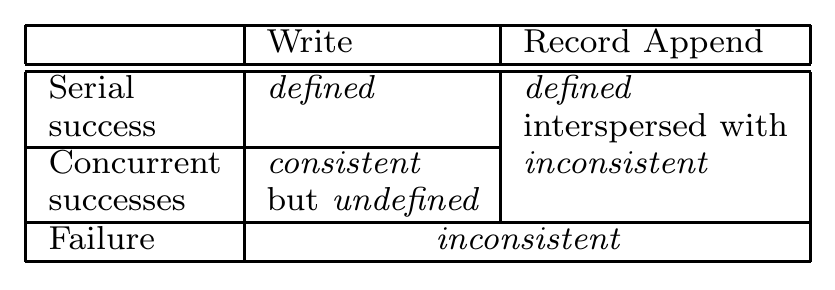
\includegraphics[width=0.95\columnwidth]{figures/original/gfs-table-1-file-region-state.png}
  \refstepcounter{table}\label{tab:file-region-state}

  {\small\textbf{Table 1.}数据mutation后的文件区域状态}
\end{center}

数据mutation\emph{(译者注：包含write和record append)}之后，
文件区域的状态取决于mutation类型、操作是成功还是
失败，以及是否存在并发mutation。Table 1总结了这些结果。如果无论客户端
从哪个replica读取，始终都能看到相同数据，则该文件区域是consistent的。
一次文件数据mutation之后，如果该区域既consistent，并且客户端能完整看到该
mutation写入的内容，则该区域是defined的。当mutation成功且未受并发写入
干扰时，受影响区域是defined的(因此也是consistent)：所有客户端始终都会看到
该mutation写入的内容。
并发成功的mutation会使该区域undefined但保持consistent：所有客户端
看到相同数据，但这些数据可能并不反映任何一个mutation实际写入的内容。
通常，它由多个mutation相互混杂的片段组成\emph{(译者注：
consistent but undefined是concurrent successes的结果，
例如client1在offset处写入AAAA，client2在offset处写入BBBB，
有可能最终的结果是AABB，最重要的原因是mutation
可能刚好跨分片，从两个客户端的角度看来，最终write函数返回的都是成功，
写出来的结果应当是AAAA or BBBB，最后读出来却可能是AABB这样的混叠数据，
这就是未定义的含义)}。
失败的mutation会使该区
域inconsistent(因此也undefined)：不同客户端可能在不同时间看到不同的数据。
下文将说明应用程序如何区分defined区域和undefined区域。应用程序无需进一步
区分undefined区域的不同种类。

数据mutation可以是\textbf{write}或\textbf{record append}。写入会
在应用程序指定的文件offset写入数据。即使存在并发mutation，\textbf
{record append}也会至少一次\emph{(译者注：这里是伏笔，以后读者会
知道如何处理重复数据保证幂等性)}原子地追加数据(即“record”)，但追加offset
由GFS选择(section3.3)，相比之下，“常规”追加只是一次写入，写入位置是客户
端认为的当前文件末尾offset，GFS会将实际offset返回给客户端；
这个offset标记了一个defined region的起始位置，而该区域包含这条记录。
此外，GFS可能会在记录之间插入padding内容\emph{(译者注：原因是
record append不能让一条record跨chunk边界；如果当前chunk剩余空间不
够放下整条record，GFS就把当前chunk剩余部分填充掉，然后让客户端到下一个
chunk重新append。实现原子append的核心设计正是“一个record不能跨chunk”，只有
一个record在一台chunk上，并且依赖chunk的pipeline串行排队执行机制
才能实现“原子append”)}，或者插入重复的record。这些padding和重复的
record占据的区域被视为inconsistent区域，并且相对于用户数据量而言通常很小。

在一系列成功的mutation之后，经过mutation的文件区域保证是defined的，
并且包含最后一次mutation写入的数据。GFS通过两种方式实现这一保证：
(a)在所有replica上以相同顺序将mutation应用到某个chunk(section3.1)；
(b)使用chunk版本号检测因chunkserver宕机期间遗漏mutation而过期的
replica(section4.5)。过期replica绝不会参与mutation，也不会被master
作为chunk位置返回给请求客户端。系统会在最早的机会对它们进行垃圾回收。

由于客户端会缓存chunk的位置信息，因此在这些缓存信息被刷新之前，
客户端可能会从一个stale replica读取数据。这个时间窗口受到两个因素限制：
一是缓存条目的超时时间，二是下一次打开该文件时会清除缓存中该文件的所有chunk信息。
此外，由于我们的多数文件都是只追加的，所以stale replica通常返
回的是一个过早的chunk结束位置\emph{(译者注：如果用户append-only而不overwrite，
当stale replica可能和primary断连后，客户端实际上最多从它这感知到early EOF，
而不是outdated data，这不是特别“危险”)}，而不是过期数据。当reader重试并联系master时，
它会立即获得当前最新的chunk位置信息。

一次成功mutation过去很久后，组件故障当然仍可能损坏或销毁数据。GFS通过
master与所有chunkserver之间的定期握手识别失效的chunkserver，并通过
校验和检测数据损坏(section5.2)。一旦问题暴露，系统会尽快从有效replica恢复数据(section4.3)。只有在GFS
来得及反应之前、通常也就是几分钟内，某个chunk的全部replica都丢失时，
该chunk才会不可逆地丢失。即使在这种情况下，它也是不可用而非被损坏：
应用程序会收到明确错误，而不是损坏的数据。

\subsubsection{对应用程序的影响}
GFS应用可以通过一些简单技术适应宽松的一致性模型。这些技术原本就因
其他目的而需要，包括依赖追加而非覆盖、创建checkpoint，以及写入可自验证、
可自标识的record。

几乎所有应用都会通过追加而非覆盖来修改文件。一种典型用法是：写入者
从头到尾\emph{(译者注：使用append)}生成一个文件，并在写完全部数据后，
原子地将文件重命名为永久名称；或者定期记录已成功写入的数据量，
形成checkpoint。checkpoint还可以包含应用层校验和。\emph{(
译者注：这里的checkpoint和之前提到的master checkpoint不是一件事，
此处指的记录某一块数据的checksum和size，告诉应用层这部分数据已经可以被
读取使用，这种边处理边读取对很多应用很有帮助)}
读取者只验证和处理截至最后一个checkpoint的文件区域，因为该区域已知处于
defined状态。即使系统存在一致性和并发的问题\emph{(译者注：这里指的是
append+checkpoint的做法)}，这套做法都很好地满足了我们的
需求。与随机写入相比，追加的效率更高，也更能抵御应用程序故障。
checkpoint使写入者可以重启后断点续写，并避免读取者处理虽然已经成功写入、但从
应用程序角度看仍不完整的文件数据。

另一种典型用法是：许多写入者并发向同一文件追加数据，以生成合并结果
或充当生产者—消费者队列\emph{(译者注：很多读者会误以为增加生产者
就能提高单个文件的append速率，实际上不是的，在同一时刻某个chunk的mutation
必须经过这个时刻“仅有一个”的primary排队，所以写入速率还是受制于primary的单机
网络、磁盘瓶颈)}。\textbf{record append}的“至少追加一次”语义能够保留每个
写入者的输出。读取者按如下方式处理偶发的padding和重复record。
写入者准备的每条record都包含校验和等额外信息，以便验证其有效性。读取者
可以使用校验和识别并丢弃额外padding和record片段。如果读取者无法容忍偶发的
重复record(例如它们会触发非幂等操作)，则可以使用record中的唯一标识符将其
过滤掉。
这些唯一标识符通常本来也需要用于命名相应的应用实体，例如Web文档。
这些record I/O相关功能(除了重复record删除之外)，都被封装在我们的
应用共享的库代码中，并且也适用于Google内部其他文件接口实现。借助这
些机制，同一串record，加上少量罕见的重复record，总是会被交付给
record reader。
